\documentclass[12pt]{article}

\usepackage{fullpage}
\usepackage{graphicx, rotating, booktabs} 
\usepackage{times} 
\usepackage{natbib} 
\usepackage{indentfirst} 
\usepackage{setspace}
\usepackage{grffile} 
\usepackage{hyperref}
\usepackage{adjustbox}
\usepackage{amsmath}
\usepackage{siunitx}
\usepackage{multirow}
\setcitestyle{aysep{}}


\singlespace
\title{\textbf{Collective Action or Exchange?: Framing International Cooperation in Alliance Politics}}
\author{Joshua Alley
\footnote{Postdoctoral Research Associate, the University of Virginia.}
\footnote{I am grateful to Alessando Del Ponte, Matthew Fuhrmann, Hyeran Jo, Erik Lin-Greenberg and Erik Peterson as well as participants in the 2020 Democratic Statecraft Lab Research incubator and 2019 Oskar Morgenstern Fellowship Colloquium for comments on earlier drafts.}}
\date{\today}

\bibliographystyle{apsr}

\begin{document}

\maketitle 

\doublespace 

\begin{abstract}
How does using different arguments to explain the consequences of international cooperation affect public attitudes towards international institutions? 
In this paper, I argue that there are two general ways to portray international cooperation--- collective action and exchange. 
I explain how using each argument to frame allied military spending affects public opinion towards the North Atlantic Treaty Organization (NATO) in the United States. 
I expect that explaining low allied military spending relative to the United States as the result of free-riding in a collective action problem reduces public favorability towards NATO and willingness to cooperate with allies. 
Framing low allied spending as the result of an exchange of protection and influence between NATO members and the United States increases favorability and support for cooperation, however. 
I test this claim with a text analysis of elite rhetoric towards NATO and a survey experiment on attitudes toward NATO in the US public. 
A pretest of the survey on Mechanical Turk finds mixed support for the argument. 
My findings provide evidence about how political framing shapes public attitudes towards international cooperation. 
\end{abstract}


\newpage 


\section{Introduction}


% Examples to start
In 2016, Barack Obama complained that ``Free riders aggravate me'' and US allies ``have to pay your fair share.'' 
Donald Trump has been more strident in criticizing US allies, especially the North Atlantic Treaty Organization (NATO). 
In June 2018, Trump wrote to Belgium that: ``it will become increasingly difficult to justify to American citizens why some countries continue to fail to meet our shared collective security commitments.''
Other politicians and foreign policy elites dispute this collective portrait of alliances by emphasizing that the United States receives other benefits besides collective security from alliance participation. 
%In his resignation letter, James Mattis wrote that: ``While the US remains the indispensable nation in the free world, we cannot protect our interests or serve that role effectively without maintaining strong alliances and showing respect to allies.''\footnote{\url{https://media.defense.gov/2018/Dec/20/2002075156/-1/-1/1/LETTER-FROM-SECRETARY-JAMES-N-MATTIS.PDF}} 
\citet[pg. 129]{RappHooper2020} argues that the US ``alliance system also lowered the cost of US political and military action worldwide.'' 
In a 1999 lecture, John McCain claimed that: `` if we must bear the greatest share of our mutual defense, then our allies must pay as much attention to our concerns, in and out of Europe, as we must to theirs.''\footnote{\url{https://www.k-state.edu/media/newsreleases/landonlect/mccaintext399.html}} 


% Generalize to other areas of international cooperation
%Such divergent rhetoric about alliances is present in other discussions of international cooperation.
%Discussions of trade, climate change, and other multilateral institutions also contained rhetoric of collective action or exchange and differentiated benefits. 
%These debates and related political rhetoric could affect public attitudes towards international cooperation by framing the sources and consequences of cooperation. 


% introduce the question and make my claim 
This competing rhetoric about alliances raises an important question; how do different portrayals of cooperation and its consequences affect public attitudes towards international institutions? 
In this paper, I identify two general ways to describe the basis of cooperation in international institutions and explain how using these arguments changes public attitudes. 
The first explanation employs a collective action logic and portrays institutional participation as a contribution to the common good. 
The second explanation emphasizes exchange between states, where cooperation provides differentiated benefits.
Each argument provides a different frame for international cooperation, which may change public opinion \citep{ChongDruckman2007}.  


The divergent processes of the two arguments affect public attitudes towards international cooperation by activating different intuitions and heuristics.   
Relative to a neutral presentation, framing international cooperation in terms of collection action activates conditional cooperation norms and exploitation concerns, which reduces can then support for cooperation in the face of perceived violations. 
Framing international cooperation as an exchange between states is more likely to increase or maintain public support for international cooperation, however. 
Exchange implies reciprocity based on mutual and heterogeneous benefits, which increases the robustness of public support for international cooperation. 


% note and justify emphasis on alliance politics
While this general argument may apply to cooperation in issues such as trade, climate change, and international institutions, this paper explores the consequences of framing international cooperation for international alliances. 
I examine alliance politics because competing frames are obvious in discussions of the benefits and burdens of alliance participation. 
Alliance politics scholarship is divided between public goods and bargaining models, and there is substantial heterogeneity in how foreign policy elites describe alliances, as the earlier quotes imply. 
For example, debates over the future of US grand strategy contain two distinct perspectives on alliances, which rely on different arguments. 
Advocates of a restrained US foreign policy often argue that US allies do not contribute enough to their own security in alliances, which then increases US defense spending \citep{Preble2009, Posen2014}.
Proponents of continued deep engagement dispute this collective action understanding of alliances and claim that the US gains substantial benefits from alliance participation \citep{BrooksWohlforth2008, BrandsFeaver2017}. 


% specific test
I examine the argument in two ways.
First, I conduct a text analysis of how US political elites frame defense spending in NATO using word embeddings.  
Then I conduct a survey experiment on public attitudes toward NATO in the United States.
The experiment describes low military spending by other NATO members relative to the United States in three ways and then asks a series of questions about individual opinions on NATO.
The first frame uses free-riding in a collective action problem to explain low allied military spending \citep{OlsonZeckhauser1966}.
The second frame explains low military spending as the result of an exchange where the US gives protection and gains foreign policy influence \citep{Morrow1991}.
A neutral frame with no explanation of allied military spending is the reference category for the two competing frames.


% Preview the findings
The text analysis finds two general frames are present in elite rhetoric about alliances. 
When US politicians discuss NATO and collective terms, they emphasize shared commitments and responsibilities. 
But when US politicians discuss influence in NATO, they are more likely to emphasize allied support. 
As a result, I an approximation of the ideal frames I use in the survey experiment is present in actual rhetoric. 
A pre-test of the survey experiment on Mechanical Turk finds some evidence that exchange framing increases favorability towards NATO and support for cooperation, but no evidence that collective action framing affects attitudes towards NATO. 


% Detail contribution: start with academic models
The argument and findings have four general implications.
First, I present indirect evidence whether regular condemnations of allied ``free-riding,'' most recently by Donald Trump, could affect public attitudes toward international cooperation, which adds to the rich literature on political rhetoric and public opinion in the United States.  
Using different explanations to frame international cooperation is a novel mechanism for understanding individual attitudes towards international institutions and cooperation. 
Existing scholarship on international economic cooperation, especially trade, uses economic interests e.g. \citep{Rogowski1987, MaydaRodrik2005} or perceptions of the costs and benefits \citep{Hainmueller2006, MansfieldMutz2009, RhoTomz2017} to explain public attitudes. 
In the domain of international institutions, \citet{Edwards2009} uses a mix of economic and ideological factors to predict support for the IMF, World Bank and WTO in developing countries and \citet{BearceScott2019} argue that individual economic concerns affect attitudes toward international institutions. 
These studies and other surveys on public attitudes towards international institutions use neutral questions \citep{KayaWalker2014, DellmuthTallberg2015}.
Neutral questions avoid leading respondents, but they do not correspond to how political actors discuss international institutions, which is a key source of public information, as the media partially transmits elite foreign policy frames \citep{BaumPotter2008}. 
Politicians, the media and other foreign policy elites frame international cooperation with different explanations to advance their goals, so common sources of information about international institutions are more slanted than the typical survey question.  


% Taking public goods and framing out of the lab
Second, the findings broaden our understanding of framing effects and may apply to cooperation beyond alliance politics and international relations.  
Most frames in survey experiments on international security examine public support for using force, but this experiment addresses interstate security cooperation. 
More generally, a vast literature examines how individuals view and contribute to collective action in laboratory settings e.g. \citep{Ostrometal1992, GachterFehr1999, Houseretal2008, Aimoneetal2013}. 
Framing is a common and powerful manipulation in these laboratory experiments, and I show how it affects attitudes towards cooperation outside the lab. 


Third, I identify a heretofore unacknowledged consequence of ideas in international relations. 
As \citet[pg. 50]{BoettkeAligica2009} write, ``Ideas set into motion actions, ideas give solutions but they also generate new problems and challenges.''
Existing research shows that ideas shape how leaders understand the costs and benefits of different policies \citep{Morrison2012, Morrison2016} and can give leaders a means of justifying their preferred policy \citep{Parsons2002}.
The same is true of the public--- exposure to different academic and popular explanations of the consequences of international cooperation affects public attitudes.


Last, this paper contributes to our understanding of the domestic politics of alliances \citep{Lobell2004, Mattes2012a}.
Public attitudes towards international institutions are important, especially in democracies, where public support can restrict leaders' policy choices \citep{Putnam1988, Fearon1998, LevenduskyHorowitz2012, Williams2013, Levyetal2015}. 
Because public attitudes shape the willingness of leaders to use force \citep{Tomzetal2020} and alliances are formal efforts to establish credible commitments of military intervention \citep{Morrow2000}, public perceptions of allies affect the credibility of the alliance. 
If elites use frames that raise the fear of exploitation by allies, subsequent changes in support for fighting alongside allies may undermine the alliance itself.  


This paper proceeds as follows. 
First, I explain how framing international cooperation in terms of collective action or exchange affects public attitudes towards international alliances. 
In the second section, I present a text analysis of elite rhetoric towards alliances that shows some evidence of collective action and exchange frames. 
Then, I describe the design and results from a survey experiment on US attitudes towards NATO that tests three predictions from that argument. 
Last, I offer some concluding thoughts for scholars and policymakers. 


\section{Argument}


% Outline the argument
I use evidence from laboratory experiments on cooperation between individuals to establish the foundations of attitudes towards international cooperation under different frames. 
First, I explain why framing could affect public attitudes towards cooperation.
Following that, I describe cooperation in alliances and disputes over why US allies spend a smaller share of their resources on the military.  
Then I describe the consequences of collective action and exchange framing for public support of alliances. 
I also explain how foreign policy information and partisanship may modify the effect of framing. 


What produces different frames for international cooperation? 
Frames are ways actors present information, and they often employ an explanation. % expand definition if needed
One can describe cooperation with either collective action or exchange reciprocity, and when actors dispute the underlying ``game'' behind cooperation, this framing is feasible, influential and political.  
Given disagreements over how the world works, political elites have more freedom use frames that advance their goals and interests. 
Framing is political because frames define whether a problem exists, and suggest a corresponding set of solutions.\footnote{Solving a collective action problem requires careful attention to institutional rules \citep{Ostrom1990} or judicious use of select incentives \citep{Olson1972, Hardin1982}.
On the other hand, cooperation through exchange requires attention to other contracting issues \citep{Williamson1985}.}  
After framing cooperation, political elites can then advocate policies that match their interests and agenda.
Any solution or policy decision, including maintaining the status quo, has distributional consequences. 
Sanctioning institutional participants for free-riding in the face of an ostensible collective action problem will benefit some actors more than others, for example.


% Framing int'l cooperation has two audiences
When elites apply frames to international cooperation, they reach international and domestic audiences. 
Thus public framing is part of a two-level game \citep{Putnam1988}. 
In this paper, I focus on the domestic level. 
For example, collective action frames are often intended to shame or encourage other states to cooperate. 
But public framing of international cooperation also reaches domestic audiences and can affect public opinion. 


% Discuss why framing can work
Adopting different frames for international cooperation affects public attitudes for two reasons. 
First, lab experiments provide ample evidence that how researchers frame cooperative games affects affects individual attitudes and behavior. 
Scholars have explored a wide range of frames for a common public goods game, which they usually present as generic investment or decision-making. 
In the voluntary contribution mechanism game, individuals can invest experimental tokens in public or private accounts, and the whole group benefits from public investments. 
Maximal investment in the public good is the Pareto optimal choice, but individuals have incentives to defect, which creates a collective action problem.
Framing impacts cooperative behavior in the lab through different subjective understandings of the underlying game \citep{Cookson2000, CartwrightRamalingam2019}. 
Changing the frame alters the weight people give particular values while forming opinions \citep{ChongDruckman2007} and beliefs about other players \citep{Dufwenbergetal2011}.
The power of framing in the lab should apply elsewhere, because the lab and field have a common psychological base. 


Second, the public has little information about international affairs and cooperation.
Limited information gives frames more power \citep{Druckman2001}, as it makes public opinions more malleable. 
Different subjective understandings from frames in the lab occur when participants do not grasp the ``true'' underlying game. 
This gives researchers and other participants the freedom to frame.
Thus, framing depends on limited information and the presence of multiple plausible explanations of how the world works, and can affect how people view cooperation.  


\subsection{Framing Alliance Politics}


% Alliance politics here
I explore the consequences of framing international cooperation in alliance politics because frames match real-world debates and could change public attitudes.  
Different frames are possible in alliance politics because elites present cooperation in competing ways and the public has little knowledge of alliance politics. 
First, it is obvious that US allies spend a smaller share of their gross domestic product on defense expenditures compared to the United States, but elites disagree about why. 
Exchange and collective action models offer different ways to explain low military expenditures.
Therefore, each argument provides a different frame for alliance politics. 
\citet{OlsonZeckhauser1966} and \citet{SandlerHartley2001} offer two well-known models where security from alliances is partially or totally a public good.
Public goods models explain low allied defense spending using a collective action problem, where small states free-ride on larger partners. 
Exchange-based models argue that allies may lower defense spending because they give up foreign policy autonomy in exchange for protection \citep{Morrow1991}.
Rather than contribute to a collective good, alliance members exchange different benefits as junior partners gain security and senior partners gain influence. 


The public also has little information about alliances, so alliance politics meets a key criterion for frames to affect public attitudes. 
Alliances can be salient in domestic politics when they engage promises of military support, but the public has limited information about alliances otherwise. 
Models of alliance politics are disputed by elites and unknown to the public, so different frames are possible and could alter subjective beliefs.
Inasmuch as the public does not have ready-made frameworks to conceptualize cooperation in alliances, they will rely on heuristics and intuitions to make sense of information from elite cues \citep{BaumPotter2008}.\footnote{I will examine whether individuals with more foreign policy knowledge are less sensitive to framing, as \citet{Druckman2001} claims.} 


Within alliance politics, I further focus on public opinion towards the North Atlantic Treaty Organization (NATO). 
Collective action and exchange frames are already present in discussions about military spending by NATO members, which draw on the broader theoretical division in models of alliance politics.
\citet{Lanoszka2015} asserts that NATO reflects a bargain where American protection is contingent on foreign policy support and nuclear non-proliferation, so low allied spending is not free-riding. 
Other researchers claim that low allied spending is the result of free-riding, however e.g.\citep{OlsonZeckhauser1966, PluemperNeumayer2015, KimSandler2019}.
Therefore, the argument addresses how framing allied military spending affects public favorability towards NATO, willingness to fight for a NATO ally, and support for leaving the alliance in response to low allied spending. 
Explicitly analyzing NATO has two advantages.
First, when the US public thinks of alliances, NATO is the most likely subject, so considering attitudes towards NATO has less risk of confounding from implicit associations. 
Second, examining NATO allows me to compare the theoretical frames with standard survey results.


% Introduce a neutal baseline
I compare the collective action and exchange frames to a neutral presentation of allied defense spending. 
A neutral presentation of NATO with no explanation of why individuals observe a given consequence of international cooperation contains no framing elements. 
Neutral framing thus approximates baseline attitudes without additional information from a frame. 


% discuss the consequences of adopting a collective action frame
% Mechanism one here
Relative to a neutral frame, I expect that using collective action to explain allied defense spending will reduce public support for cooperation in NATO through two mechanisms.
First, collective action frames raise fears of exploitation. 
Individuals do not want to be taken advantage of. 
Lab experiments on collective action corroborate the intuition that individuals dislike receiving a sucker's payoff. 
Cooperative individuals are often willing to punish free-riders, even at substantial cost to themselves \citep{FehrGatcher2000, Seftonetal2007}.\footnote{Such sanctions can promote cooperation \citep{Guererketal2006}, but punishment is not always effective \citep{Houseretal2008} or efficient \citep{Pageetal2005, Seftonetal2007, Randetal2009}.}


% Mechanism two here
Second, collective action framing of allied defense spending reduces public support for NATO by activating conditional cooperation norms. 
Substantial evidence from public goods experiments suggests individuals are conditional cooperators \citep{Chaudhuri2011}.
Defection in the lab often generates social disapproval \citep{GachterFehr1999, Cubittetal2011a}, and may present a moral dilemma as individuals fear violating norms \citep{Nielsenetal2014}. 
So long as other players contribute to the collective good, individuals are willing to cooperate.\footnote{Beliefs about cooperation and cooperative behavior in the lab depend on other players' contributions \citep{FischbacherGachter2010}.}


% State collective action hypothesis
Under a collective action frame, low allied military spending generates fear of exploitation and violates conditional cooperation norms.
A collective action frame defines low allied spending in terms of the common good and opportunism, so low allied defense spending violates the purpose of cooperation in the alliance and leaves the US to bear a disproportionate burden. 
Therefore, collective action framing of low allied defense spending will reduce public favorability towards the NATO. 


I also expect that collective action framing will decrease willingness to intervene militarily on behalf of allies, and increase support withdrawing from NATO. 
Abandoning allies by leaving NATO may reduce US welfare, but aversion to exploitation and anger at violating conditional cooperation norms should overcome these costs.   
Also, if respondents believe that allies violated conditional cooperation norms, they will be less willing to cooperate through military support. 


% discuss the consequences of employing an exchange frame
Using exchange to explain allied military spending has different consequences for public attitudes. 
Explaining allied military spending through a mutually beneficial trade is less likely to raise a sense of exploitation, because low allied defense spending is no longer presented as an inadequate contribution to collective security. 
It also matches a different underlying psychological tendency. 
People are used to exchanging different favors.
This willingness to engage in exchange reciprocity is present even in impersonal laboratory experiments \citep{McCabeetal1996}. 
Individuals understand that cooperation can yield a larger total prize, which facilitates reciprocity and social exchange \citep{Hoffmanetal1998}. 


With exchange, both sides benefit from cooperation, but not necessarily in the same way. 
Both parties to an exchange gain something, but their gains need not be equivalent or proportionate to make trading worthwhile. 
Thus, if individuals believe that they or their country benefits from cooperation, even if partners do not behave in the same way, they will be more likely to support cooperation. 
For example, explaining the consequences of protectionism increases support for trade liberalization by individuals who might benefit \citep{RhoTomz2017}.\footnote{Of course, if individuals believe an exchange is unfair, they will not support it.}


% state the exchange hypothesis: Greater or equal
Exchange framing of allied military spending should increase or maintain individual favorability towards NATO, relative to a neutral frame. 
With the understanding that cooperation produces heterogeneous benefits, low allied military spending is not a barrier to approval. 
The exchange frame might also activate conditional cooperation norms and thereby bolster willingness to support allies militarily. 
When low allied military spending does not reflect a lack of cooperation, respondents will be more willing to support fulfilling US obligations. 
Last, support for leaving the alliance should also fall, because respondents will not believe it is necessary.  


Thus, the argument produces three general hypotheses. 
First, collective action and exchange frames should have different effects on favorability towards NATO. 
Collective action framing of allied military spending will decrease favorability, but exchange framing should increase favorability. 

% Prediction 1
\begin{quote}
\textsc{Hypothesis 1}: Compared to the neutral frame, respondents will have less favorable views of NATO in the collective action frame, and more favorable views in the exchange frame.  
\end{quote}

Second, framing allied military spending will change support for military intervention on behalf of NATO members. 
Given conditional cooperation norms and concern with exploitation, collective action framing will reduce public support for intervention. 
Exchange framing should increase support for intervention, however. 

% Prediction 2
\begin{quote}
\textsc{Hypothesis 2}: Compared to the neutral frame, fewer respondents will support military intervention to defend a NATO member in the collective action frame, and more respondents will support intervention in the exchange frame. 
\end{quote} 


Finally, framing will affect attitudes toward policy responses to allied military spending. 
Under collective action, more respondents will favor leaving the NATO treaty. 
But low spending should be perceived as less problematic in the exchange frame, which will make respondents less likely to support leaving the alliance entirely. 


% Prediction 3: this is the weak link. 
\begin{quote}
\textsc{Hypothesis 3}: More respondents will support leaving NATO in response to low allied military spending in the collective action frame, compared to the neutral frame.
\end{quote}


The first response question deals with attitudes towards NATO, while the second and third questions deal with support for particular actions. 
A priori, I expect that framing will have a larger effect on favorability towards NATO than attitudes towards policy. 
Attitude changes have fewer cost and countervailing considerations than policy changes. 


These hypotheses have two further implications. 
First, support for alliance cooperation should be higher in the exchange frame than in the collective action frame. 
Second, if my argument is correct, framing works because the public has limited foreign policy information. 
Therefore, respondents with high foreign policy information may be less sensitive to framing \citep{Druckman2001}. 
I test these conditional relationships later in the analysis. 


%discuss partisanship and pandering
Partisanship may also condition how individuals respond to the two frames. 
Republicans tend are often skeptical of international institutions and NATO, while Democrats have more favorable views.
By attributing the alliance frames to the same non-partisan think tank in the prompt, I hope to avoid partisan cues, but information about alliances may reinforce existing views. 
For example, Republican skeptics of NATO may be more sensitive to exploitation concerns in the collective action frame, while Democratic support may be further bolstered by the exchange frame. 
Again, I test this conditional relationship later in the analysis. 


Although my argument asserts that the public responds to elite cues and rhetoric, elites might instead pander to existing public attitudes.\footnote{\url{https://fivethirtyeight.com/features/is-trump-fueling-republicans-concerns-about-nato-or-echoing-them/}}
If elite rhetoric on alliances is mostly pandering, then individuals could discount the frames entirely and retain their original alliance attitudes.
This implies stable attitudes toward alliances that elites can pander to.  
Elite pandering to public attitudes towards international cooperation is unlikely for three reasons, however. 
First, \citet{Canes-Wrone2006} finds that Presidents rarely pander to the public unless they already agree with public preferences, and are more likely to match public opinion on everyday issues for voters \citep{Canes-WroneSchotts2004}.  
Second, public attitudes are not stable and exogenous to elite messaging in general \citep{Druckman2014} and low foreign policy information in the public should accentuate the importance of framing.
Third, foreign policy is not the primary concern of many voters, so elite foreign policy views and rhetoric can diverge from public attitudes with limited fear of political repercussions \citep{BusbyMonten2012}. 


In the next section, I show that elite rhetoric around NATO in the United States has content to match the two frames. 
Besides adding an important element of realism to the survey experiment, this analysis also provides insight into elite rhetoric about alliances. 


\section{Elite Rhetoric about NATO}


If elites discuss, debate and frame alliances in different ways, then these frames can reach the public. 
If the content behind exchange and collective action frames is absent from elite discussions of alliances, then the following survey experiment lacks some realism. 
While the examples in the introduction provide a sense that elites employ different frames for alliance politics, I provide more systematic evidence of such frames in this section. 


To identify different frames of NATO defense spending, I use word embeddings, with are a popular technique in natural language processing. 
Word embedding models predict the presence or absence of different words in the context around a central word. 
As such, this technique can capture semantic relationships and associations.
One application uses word embeddings to quantify the extent and type of gender stereotypes in the United States over time \citep{Gargetal2018}, while another examines ideology \citep{RheaultCochrane2020}.
Unlike topic models, which treat each document as an unstructured ``bag of words,'' word embeddings predict the context around a given word.  


To identify the rhetorical context around NATO, I use the Global Vectors (GloVe) word embedding algorithm \citep{Penningtonetal2014}.  
I fit separate GloVe models to two collections of texts where US political elites discuss NATO: one from the US Congressional Record, and the other from US Presidential archives. 
In both corpora, I include speeches that mention NATO, and apply separate models to each corpus. 
The model predicts context words for the twenty words surrounding each word in the document, and generated a vector measuring the association identifying similar words. 
Each word in the vocabulary of the documents has an associated vector quantifying its relationship with other words in the document. 
These word vectors then provide the basis for identifying frames around NATO. 


To assess the presence of frames, I identify the most similar words for combinations of ``NATO'', ``defense'', ``spending'', and two keywords that correspond to each frame. 
I include the defense and spending vectors to match the competing frames in the survey experiment, and this also limits the risk that the model picks up other discussions of spending and budgets. 
In the baseline, neutral condition, I look at the most similar words for a linear combination of ``NATO,'' ``defense,'' and ``spending'' alone.  
For collective action, I add the word ``collective'' to the baseline combination. 
To identify exchange, I examine what words are most likely in the context around the base vector and ``exchange.''
In this model, I identify the most likely words in the context, through linear relationships between the individual word vectors, which express linguistic and semantic association. 
A linear combination of NATO, defense, spending, and a key framing word provides a unique vector with the combined rhetorical context of these words. 
In these results, I highlight the most similar words in the top 20 of each vector, but remove standard English stopwords from the results. 
I present the content of the different frames in \autoref{tab:glove-vectors}.  

\begin{table}[htpb]
\centering
\begin{tabular}{llllll}
  \multicolumn{2}{c}{Neutral} & 
                                   \multicolumn{2}{c}{Collective} &
                                   \multicolumn{2}{c}{Exchange}\\ \hline
President & Congress & President & Congress & President & Congress \\ 
  \hline
defense & defense & defense & defense & defense & defense \\ 
  nato & nato & collective & nato & spending & military \\ 
  security & military & nato & security & also & nato \\ 
  spending & spending & security & allies & budget & support \\ 
  also & allies & alliance & military & mutual & allies \\ 
  military & security & military & european & commitment & also \\ 
  now & budget & also & alliance & alliance & believe \\ 
  budget & overall & spending & overall & cooperation & security \\ 
  alliance & fact & commitment & rather & security & states \\ 
  united & believe & therefore & europe & economic & united \\ 
  therefore & expenditures & strengthen & united & strategic & part \\ 
  allies & year & allies & part & expenditures & fact \\ 
  plan & now & national & believe & increase &  \\ 
  states & also & effort & states & national &  \\ 
  addition & states & budget & natos & program &  \\ 
   &  & effective &  &  &  \\ 
   &  & plan &  &  &  \\ 
   \hline
\end{tabular}
\caption{Most similar words to linear combinations of NATO, defense, and spending
                     in GloVe word embedding models of Presidential and Congressional orations about NATO.                     
         Each vector taken from the top 20 most similar words, based on cosine similarity.             
        Blank entries indicate stopwords in the vector.} 
\label{tab:glove-vectors}
\end{table}

\autoref{tab:glove-vectors} shows some rhetorical variation in how elites present NATO when different framing key words are present in discussions of NATO, defense and spending. 
The words in each vector of the table are ordered by their similarity, or how frequently they appear in a particular context. 
In general, the top words are generic alliance terms, which is unsurprising.
Spending, expenditures and budgets are present in all three contexts and across the different branches of government.  


The relative emphasis or similarity of different words changes with the rhetorical context, however.
Under a collective action frame, Presidential rhetoric emphasizes joint action and military capacity.  
Congress discusses Europe and Europeans more when using collective language for NATO.
Particularly in Presidential rhetoric, there is a clear difference between the neutral condition and rhetoric that includes the word ``colllective.''


The exchange frame is less clear, but the word embeddings contain some suggestive evidence that discussions of exchange around NATO. 
When Presidents discuss exchange and NATO, commitment and cooperation take on greater weight, and presidents are more likely to discuss economic and strategic issues. 
Congress highlights support, but there is less evidence of a consistent exchange frame in this corpus.  


All told, these estimates suggest that elite language around alliances varies with collective and exchange phrasing. 
Having established variation in the rhetorical context around NATO, I now describe the survey experiment I will use to test these predictions. 
The experiment relies on different descriptions of NATO, and asks the public about their attitudes toward NATO after treatment with different vignettes. 
I start by describing the different treatments, before turning to the outcome measures and concluding with a list of control variables. 



\section{Experimental Design}


In the survey experiment I vary descriptions of NATO and military spending by non-US alliance members in a sample of the US public. 
Each description provides a distinct frame, of either neutral, collective action, or exchange. 
The design draws on a growing literature linking political behavior and international relations \citep{Hafner-Burtonetal2017} and offers a clean test of whether changes in framing alter public attitudes towards alliances.


The treatment in the experiment is a short vignette on NATO. 
A neutral control vignette introduces NATO and mention that allies spend a smaller share of their resources on defense than the United States. 
In the second vignette, my description of NATO explains allied military spending with collective action language that highlights disproportionate US contributions.\footnote{I do not use the words ``free-riding,'' because this explicit label could activate extant preferences, specifically general aversion to free-riding.} 
The third vignette emphasizes exchange between the United States and its allies to explain allied defense spending. 


% Justify emphasis on observed case, not hypothetical scenario 
The survey focuses on NATO rather than a hypothetical alliance for three reasons. 
First, explicitly discussing NATO avoids confounding effects, which are a potential threat to inference in survey experiments, especially those with a short vignette \citep{KrepsRoblin2019}. 
Confounding occurs when respondents impute characteristics to the survey situation, and NATO is the most likely confounder in the United States. 
When public respondents think about US alliances, NATO is the most likely subject because it is the best-known international alliance.
Second, debates about the military spending of US allies are well established in NATO. 
As a result, the experiment approximates the effects of ongoing policy debates on public attitudes. 
Last, using NATO facilitates comparisons with earlier surveys.
 

Because framing has political implications, who frames NATO and allied military spending matters. 
In the vignettes below, I attribute the information about NATO to an unnamed expert with the Council on Foreign Relations, a non-partisan think tank. 
Given extensive partisan polarization, attributing information about NATO to a partisan political elite could wash out the effects of the collective action or exchange information \citep{Druckmanetal2013}. 
I now summarize the three vignettes, with the differences in italics. 
 
 
\begin{enumerate}

\item \textbf{Neutral}: The United States has an important role in the North Atlantic Treaty Organization (NATO). NATO is a military alliance where members promise to support one another in war. According to an expert at the Council on Foreign Relations, a non-partisan think tank, some NATO members spend a smaller share of their resources on the military than the United States. 

\item \textbf{Collective Action}: The United States has an important role in the North Atlantic Treaty Organization (NATO). NATO is a military alliance where members promise to support one another in war. According to an expert at the Council on Foreign Relations, a non-partisan think tank, some NATO members spend a smaller share of their resources on the military than the United States, \textit{because the United States provides a disproportionate share of security resources for the whole alliance.} 

\item \textbf{Exchange}: The United States has an important role in the North Atlantic Treaty Organization (NATO). NATO is a military alliance where members promise to support one another in war. According to an expert at the Council on Foreign Relations, a non-partisan think tank, some NATO members spend a smaller share of their resources on the military than the United States, \textit{because they support US initiatives and goals in international politics in exchange for US protection.}
 
\end{enumerate}  


After randomly assigning a vignette to each respondent, I ask three questions about their perception of the alliance, willingness to intervene on behalf of allies and the best policy response to allied military spending. 
To assess overall opinion toward the alliance, I modified a question on alliance favorability from the Pew Research Center \citep{PewNATO2020}.\footnote{The main modification is removing the don't know option, as the treatment provides more information about an alliance than a standard survey question, and don't know responses can represent a wide range of attitudes.} 
Answers to this question are the outcome of interest for Hypothesis 1. 
My question reads: \textit{Please tell me if you have a very favorable, somewhat favorable, neither favorable nor unfavorable, somewhat unfavorable, or very unfavorable opinion of NATO? that is, the North Atlantic Treaty Organization:} 
\begin{itemize}
\item Very favorable. 
\item Somewhat favorable. 
\item Neither favorable nor unfavorable.  
\item Somewhat unfavorable. 
\item Very unfavorable. 
\end{itemize}


To assess willingness to intervene on behalf of allies, I modify another Pew survey question which addresses whether the United States should use force to defend a NATO ally from Russia \citep{PewNATO2020}. 
Responses to this question are the outcome for Hypothesis 2.  
The question reads: \textit{If Russia got into a serious military conflict with one of its neighboring countries that is our NATO ally, do you think the United States should or should not use military force to defend that country?}
Possible responses include: 
\begin{itemize}
\item Yes, should use military force.  
\item No, should not use military force.   
\end{itemize}


The final question assesses Hypothesis 3 by asking about support for different policy responses to allied military spending, including leaving the alliance. 
I will ask respondents to select the best policy response from the following list of options, which will be randomly ordered. 
Willingness to withdraw from the alliance is the main outcome of interest here. 
The exact question wording is: \textit{What should US leaders do, if anything, in response to allied defense spending?:} 
\begin{itemize}
\item Nothing. 
\item Give a verbal warning.
\item Cooperate more with allies in defense planning.
\item Impose economic sanctions.
\item Withdraw from the NATO alliance. 
\end{itemize}


Because I expect that framing will have a larger effect on favorability than policy support, I randomize the order of these three questions within the experiment. 
Randomizing the order of the response questions means that responses to the attitude question should not affect policy support and vice-versa, although consistent attitudes will generate correlations between these attitudes.
As such, there is a randomization element within the framing treatment.  


The argument relies on three broad mechanisms--- exploitation aversion, conditional cooperation, and exchange reciprocity. 
To assess the role of these factors, I also asked an open-ended question where respondents have the opportunity to explain their policy preferences.
I will then analyze these responses with a structural topic model. % Add cite here.  
Responses to this question will be especially interesting for the neutral frame, as they will clarify the default understanding of alliances without any information from framing.\footnote{Currently working through this step.}


Other individual characteristics may be correlated with attitudes toward alliances and international cooperation. 
Therefore, the survey will include a standard battery of control variables, including partisan affiliation, political ideology, education, state of residence, gender and age.\footnote{I also include a manipulation check at the end of the survey.} 
I also adjust for national identity \citep{Herrmannetal2009} and foreign policy information, which I will include as pre-treatment questions. 
After an initial analysis, I examine whether foreign policy information and political partisanship modify the treatment effects.


To examine the hypotheses, I focus on the treatment effects of the exchange and collective action frames, relative to the neutral vignette. 
I start with simple difference of means tests and descriptive statistics. 
Then I move to separate regression models that adjust for salient pre-treatment factors. 
Last, I analyze all three responses in a multivariate model that adjusts for correlations between the responses. 



\section{Results} 

In this section, I present results from a pre-test of the survey experiment on a sample of US respondents from Mechanical Turk. 
Results are mixed, as a I find support for the exchange hypothesis in the context of military intervention, and largely null results otherwise.
The only departure from this pattern is a positive effect of the exchange frame on a dummy indicator of favorable opinion in a multivariate model that adjusts for correlations between the response variables.  
The consistent military intervention finding is especially surprising because military intervention is perhaps the most costly attitude of the response variables, so this result in conjunction with null effect of the treatments on less consequential responses like favorability is unexpected. 


In an ANOVA analysis, there is no clear difference in favorability towards NATO across the neutral, collective action and exchange groups. 
The same inferences are supported by a regression model that controls for other factors, including partisanship, ideology and foreign policy information.
I summarize the results from full regression specifications in \autoref{fig:mturk-res-both}. 
The left panel of the plot shows estimates from a linear regression where NATO favorability is the dependent variable. 
The middle and right panel present coefficient estimates from logit models of support for nonintervention and withdrawal from NATO respectively. 


\begin{figure}
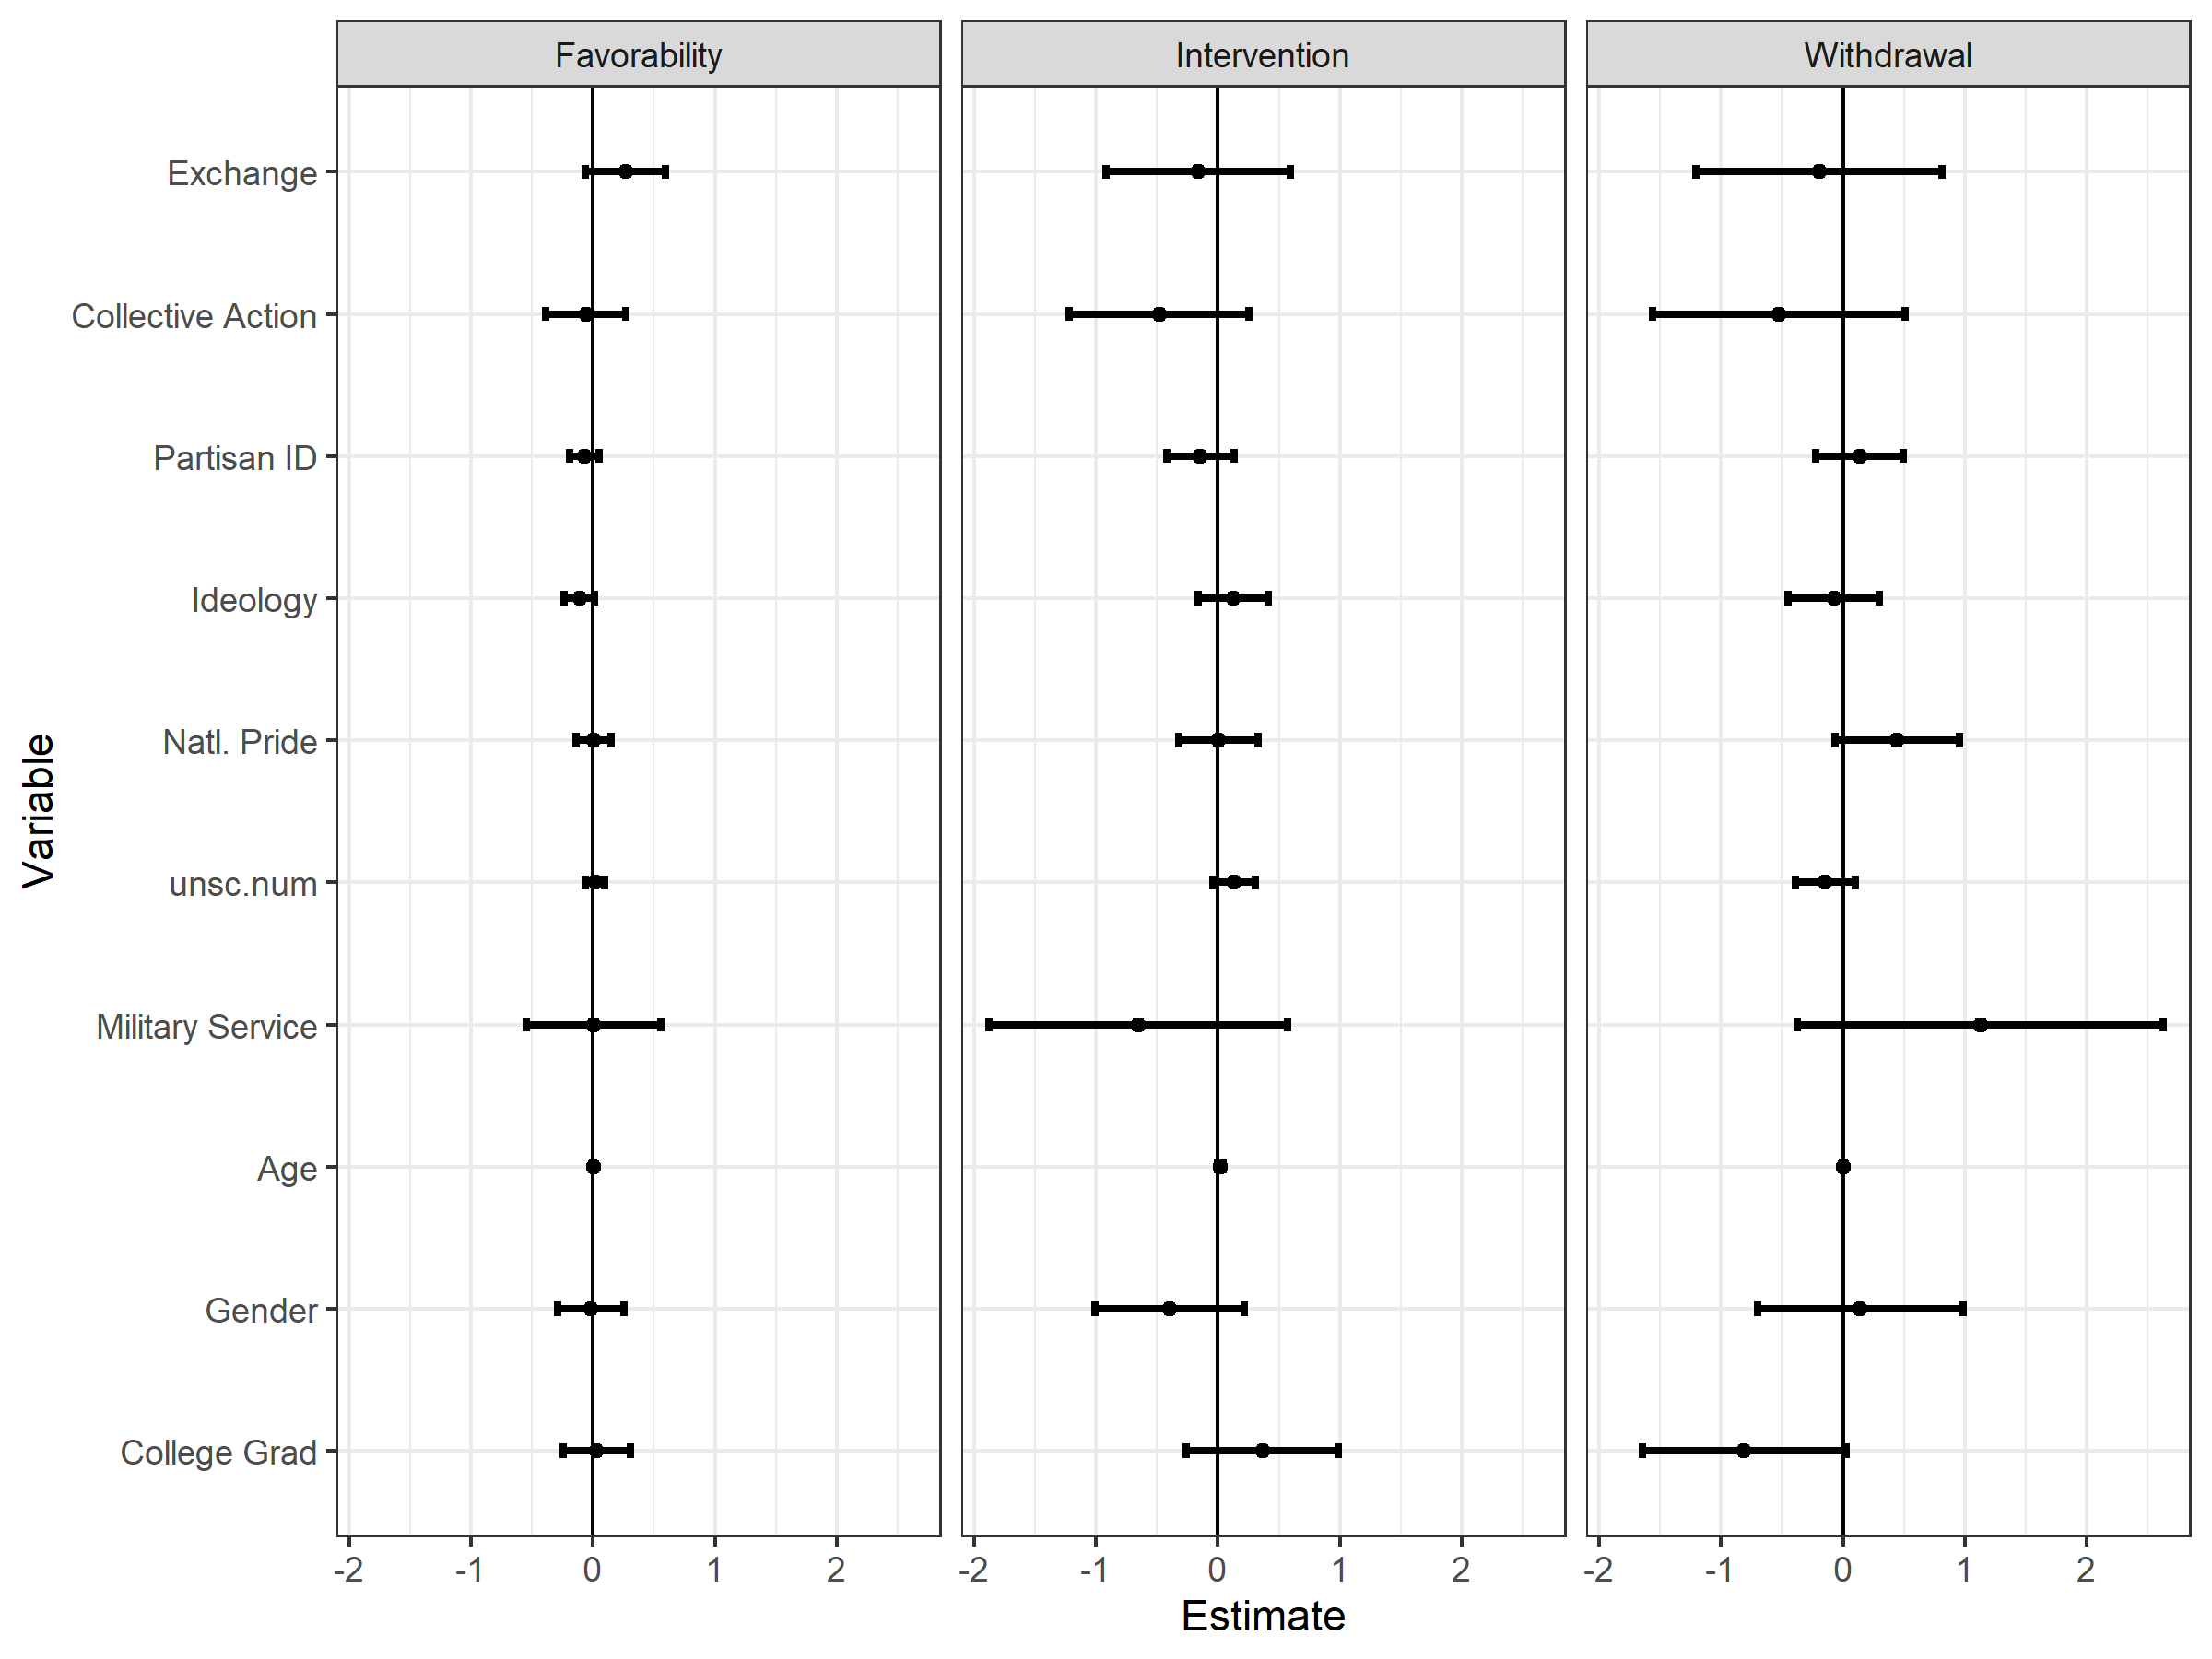
\includegraphics[width = .95\textwidth]{../figures/mturk-res-both.png} 
\caption{Coefficients from linear regression and GLM models of attitudes towards NATO in a sample of MTurk respondents from August 2020. Intercepts omitted to make the plot more legible.}
\label{fig:mturk-res-both} 
\end{figure} 


Contrary to the first hypothesis, collective action and exchange framing has  little effect on favorability towards NATO. 
Although the coefficients are both in the expected direction, their substantive impact is quite small. 
NATO attitudes are correlated with other factors, however. 
More conservative partisan affiliation and ideology both reduce NATO favorability, while national pride and past military service are both positively correlated with perceptions of NATO. 


There is some evidence that an exchange frame decreases support for nonintervention if a NATO ally is attacked, however. 
This is consistent with half of hypothesis 2.\footnote{In a one-tailed test, this effect is statistically significant at the 5\% level.}
More Republican affiliation increases support for nonintervention, while individuals with military service and more national pride are more likely to support intervention.  


Last the frames have little effect on support for withdrawal from NATO. 
There is almost no variation in support for NATO withdrawal across the exchange, collective action and neutral groups, as roughly ten respondents in each group support withdrawal.  
As a result, the estimated treatment effects are very close to zero. 
Only ideology has a clear effect on withdrawal, as more conservative ideology increases support for withdrawing from NATO. 


Therefore, evidence for the hypotheses from these three models is very limited. 
The above results do not adjust for correlations between the three response variables, however.
Favorability, attitudes towards intervention, and withdrawal from NATO should all be correlated, as individuals with favorable opinions have lower support for nonintervention and withdrawal.
Similarly, support for nonintervention and withdrawal should be positively correlated. 


Therefore, I use a generalized joint regression model \citep{Braumoelleretal2018} to model the three outcome variable simultaneously. 
This flexible modeling approach uses copulas to capture correlations in the error terms of multiple equation models. 
It does not accommodate three equations with two binary and one continuous outcome, however. 
Therefore, I translated the favorability scale into a dummy variable, where respondents that were somewhat or very favorable towards NATO received a score of one, and all others a score of zero. 


\begin{figure}
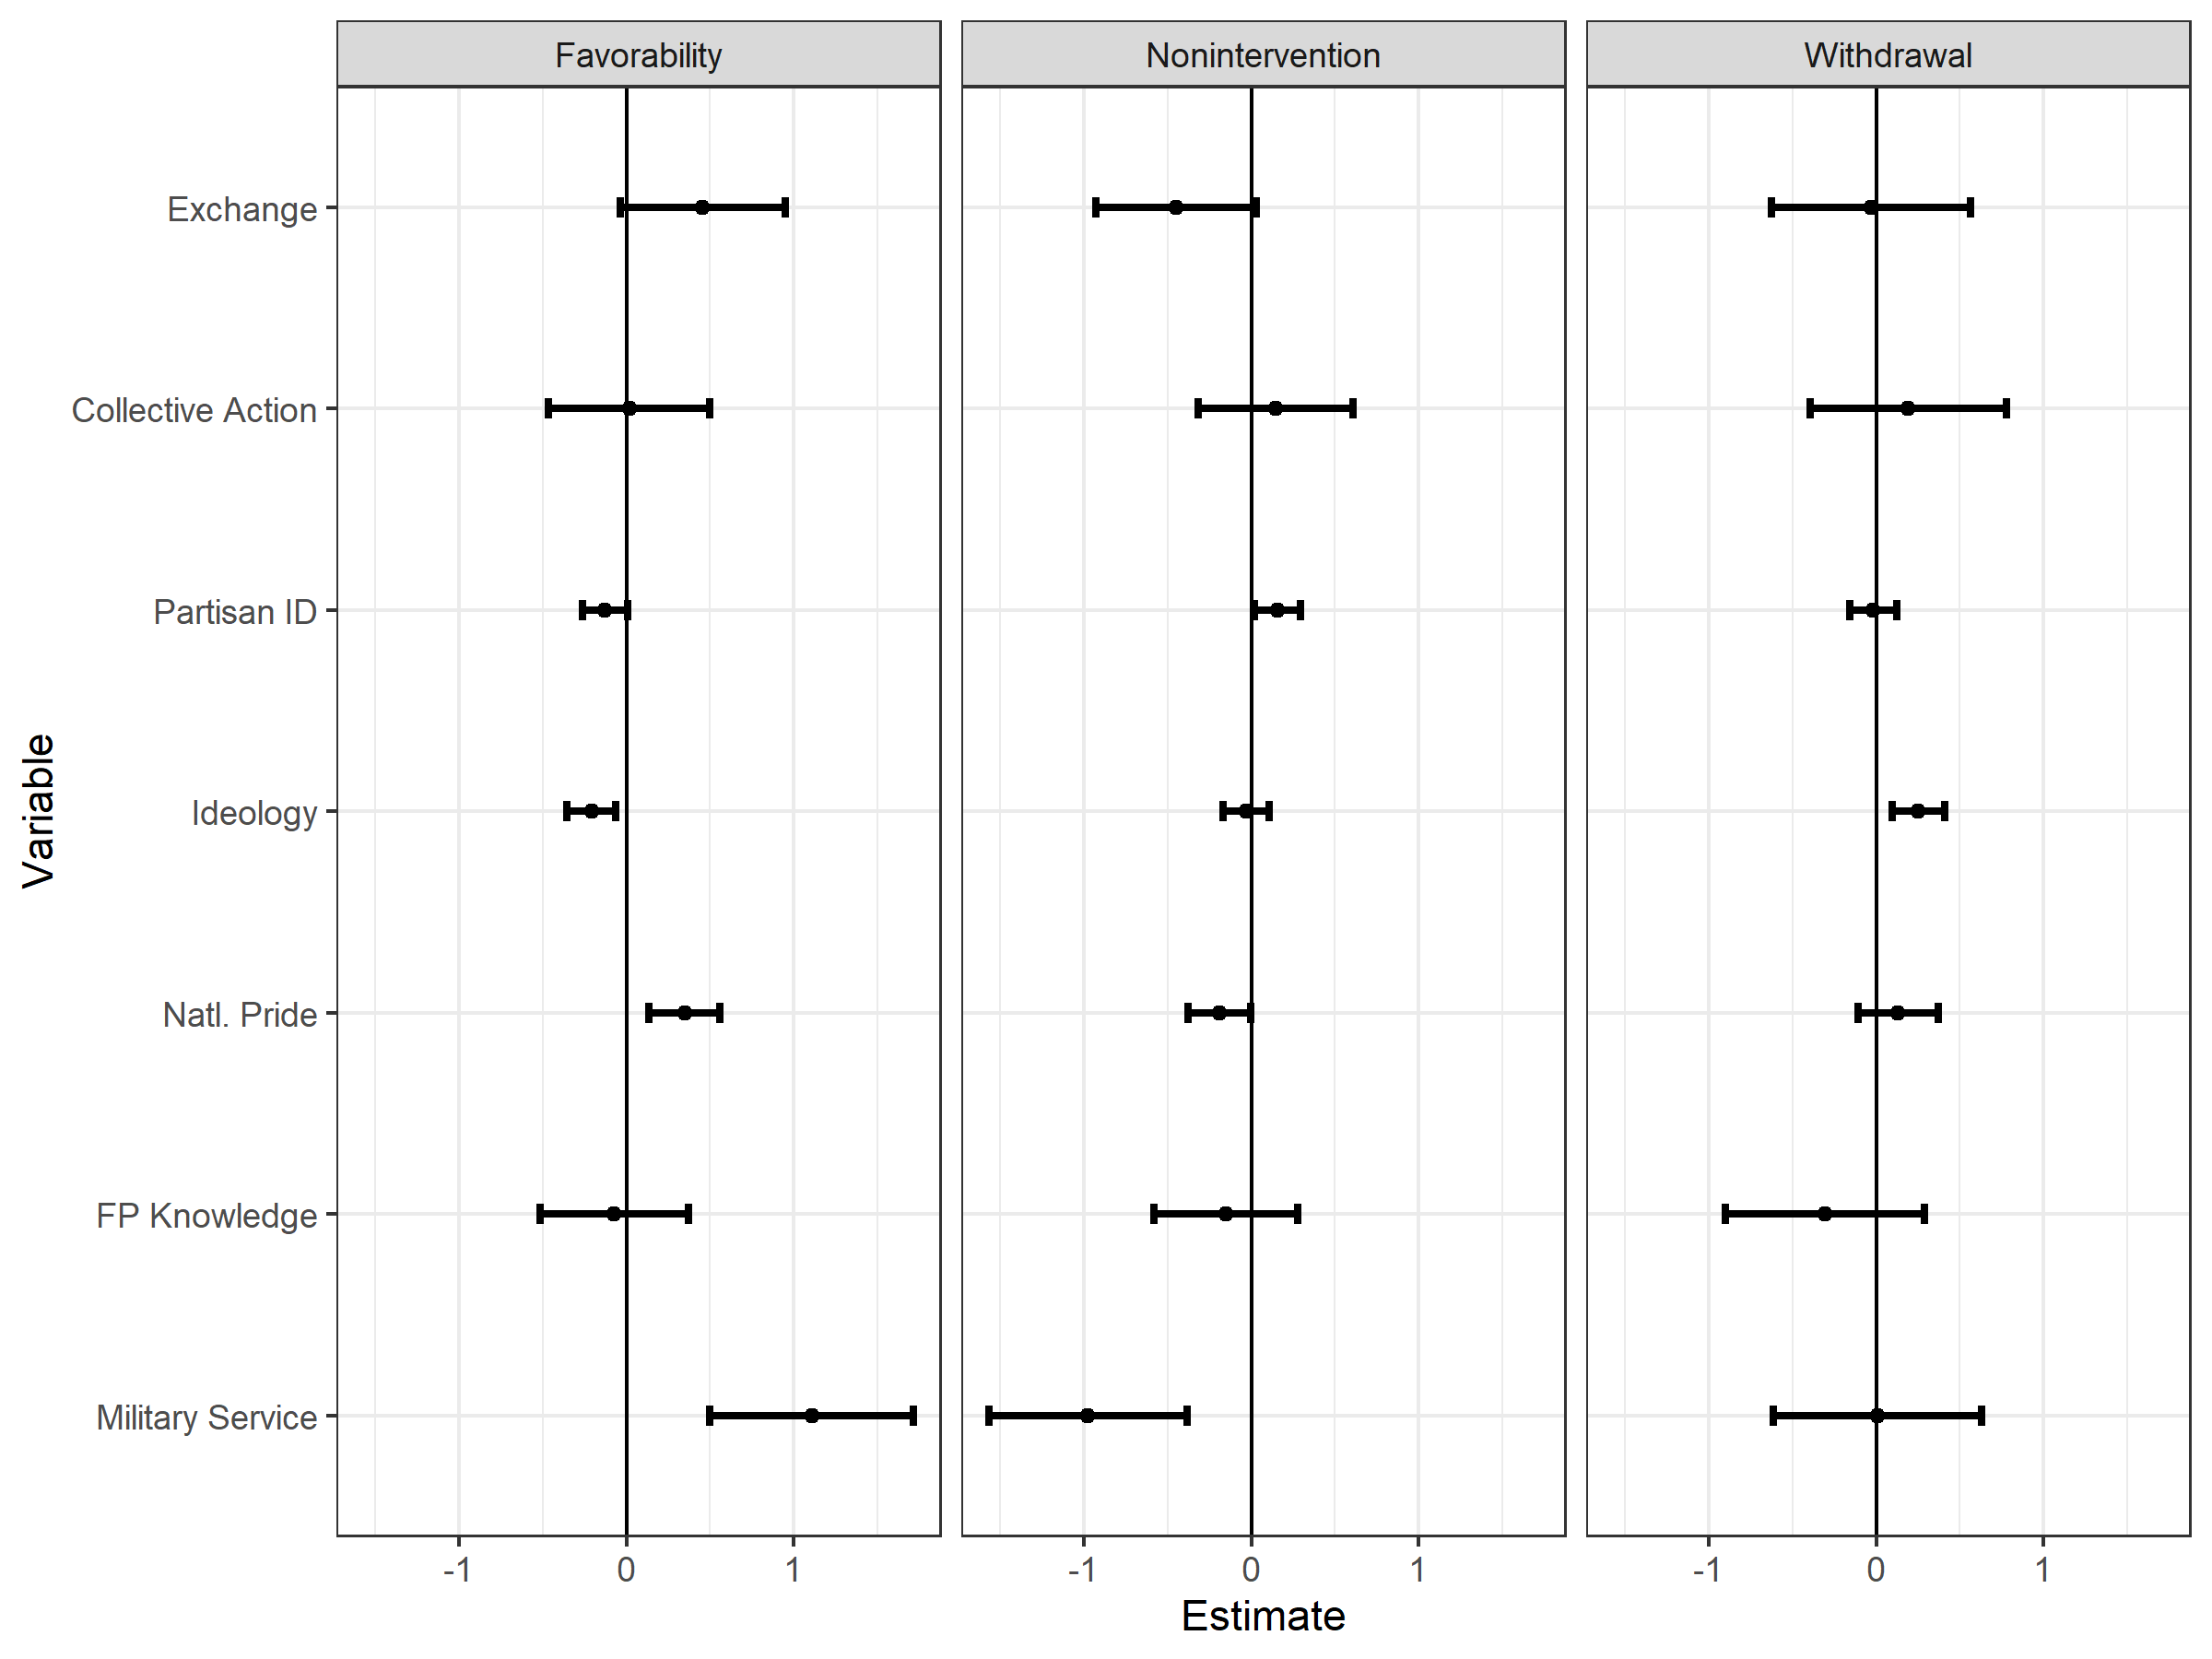
\includegraphics[width = .95\textwidth]{../figures/gjrm-res.png} 
\caption{Coefficients from a trivariate probit model of attitudes towards NATO in a sample of US MTurk respondents from August 2020. Intercepts omitted to make the plot more legible.}
\label{fig:gjrm-res} 
\end{figure} 


I plot the results of the trivariate probit model in \autoref{fig:gjrm-res}. 
The inferences from this model are very similar to the univariate specification, with a key exception. 
After adjusting for the correlation between favorability and the other outcomes, there is a positive association between the exchange frame and favorable attitudes towards NATO.\footnote{Again, I reject the null at the 5\% level in a one-tailed test.}
Exchange framing increases the likelihood an individual expresses a somewhat or very favorable opinion of NATO.  
The inference may be driven by translating the favorability measure into a dummy, however, as a I make a similar inference with a single-equation logit model.  


The correlations between different survey responses are largely as expected.
Favorability is negatively correlated with support for withdrawal, and the estimated correlation ranges from -.6 to -.2. 
Similarly, the error term correlation between favorable attitudes towards NATO and support for nonintervention ranges from -.71 to -.17.
The correlation between support for nonintervention and withdrawal is largely positive, but more uncertain, as it falls between -.14 and .39. 



\section{Discussion and Conclusion} 


% Summarize results
In summary, most of the survey experiment results in a Mechanical Turk sample with roughly 60 observations per treatment group do not match my expectations. 
The collective action treatment has little effect on attitudes towards NATO, relative to a neutral frame with no explanation of allied military spending. 
The exchange frame increases support for military intervention, and increases the likelihood of a favorable response. 


% discuss possible limitations one by one. 
In the following discussion, I offer three explanations for these results. 
The first, and most straightforward is that the argument is wrong, or at least requires refining. 
The exchange results suggest that the argument is not entirely incorrect, however. 


% CA is default understanding
Another possible explanation is that collective action is the default understanding of alliance politics in the US public. 
As a manipulation check, I asked respondents why NATO allies spend less on the military then the United States. 
I included a variant of this question for respondents in the neutral vignette, which did not include any explanation from the fictitious foreign affairs expert. 
As \autoref{fig:neutral-mech} shows, a plurality of respondents in the neutral frame attributed low allied spending to the collective action mechanism. 
Furthermore, the exchange treatment had more problems with respondents failing the manipulation check. 
Thus, the limited impact of the collective action treatment may reflect pre-treatment of US respondents with collective action explanations by politicians. 


\begin{figure}
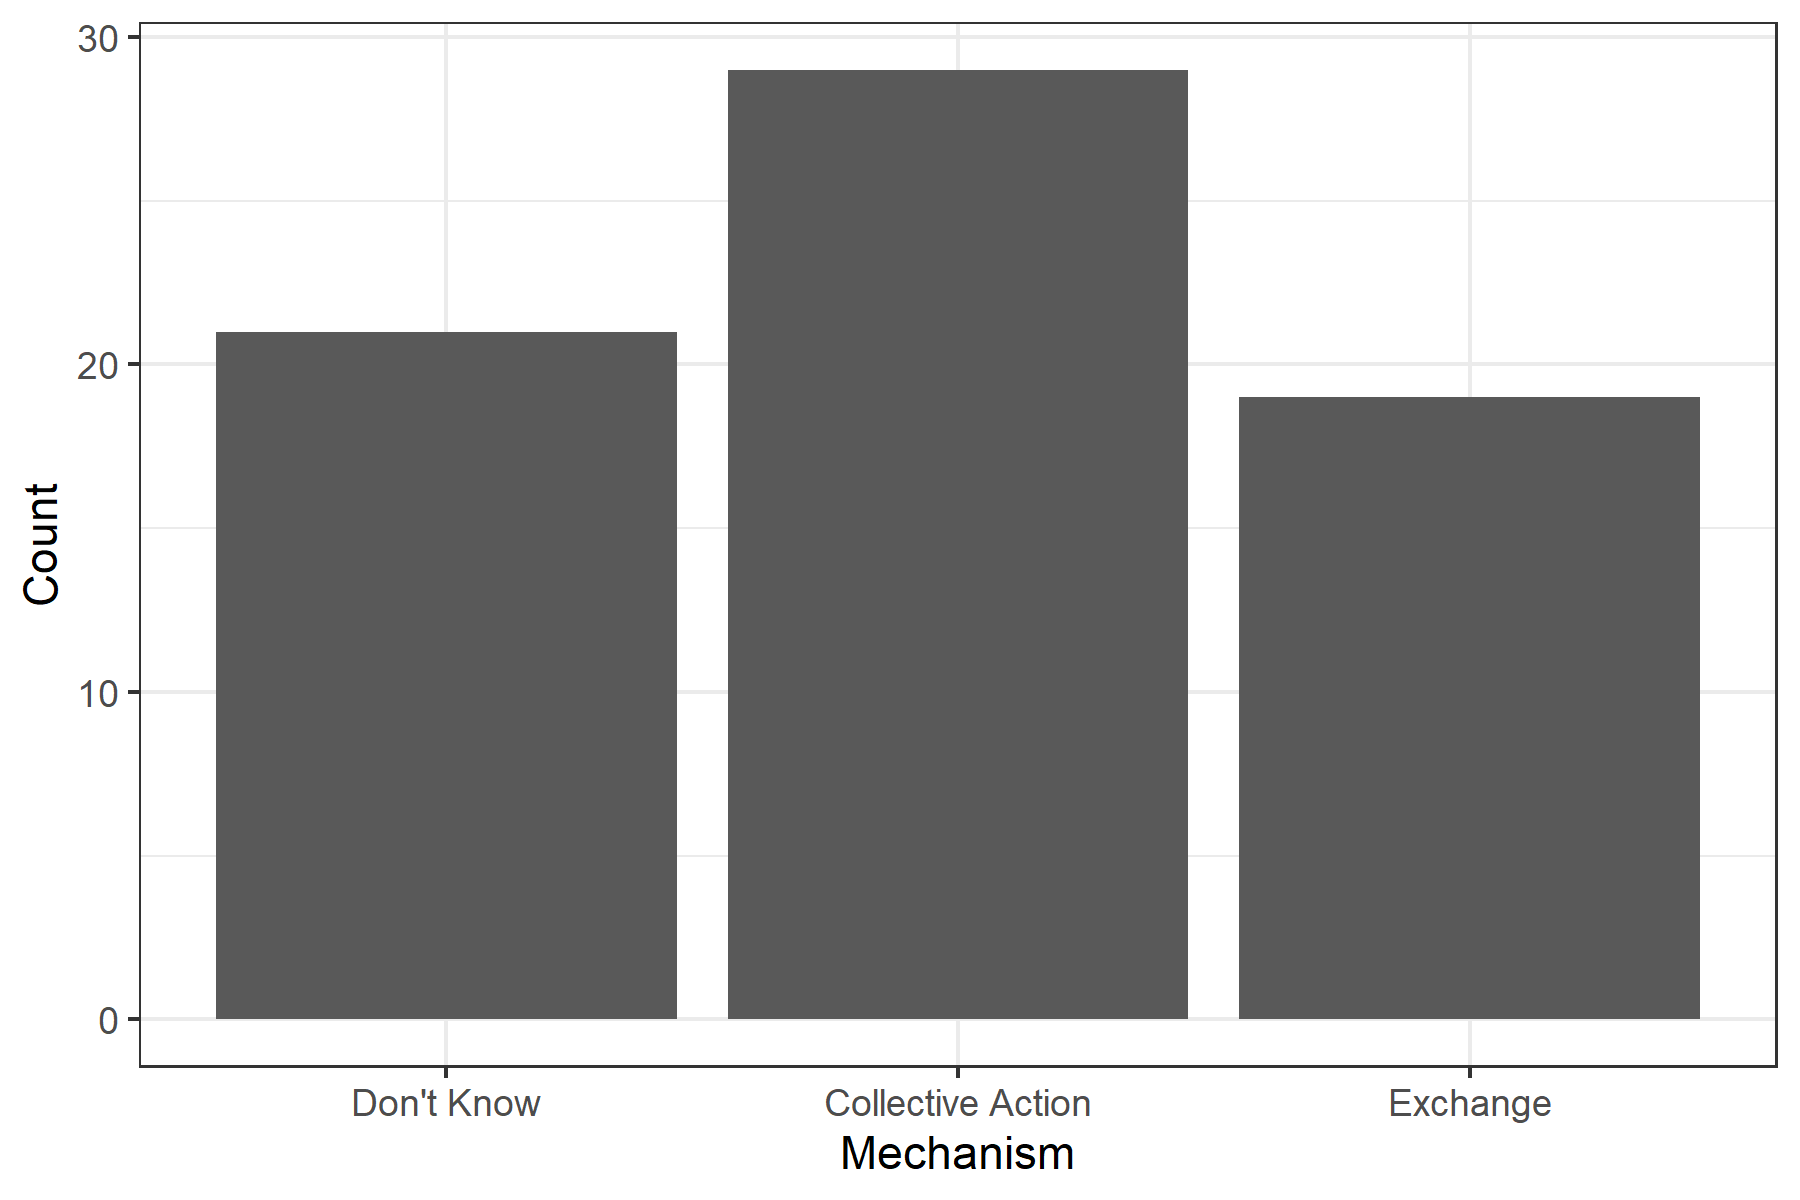
\includegraphics[width = .95\textwidth]{../figures/neutral-mech.png} 
\caption{Coefficients from a trivariate probit model of attitudes towards NATO in a sample of US MTurk respondents from August 2020. Intercepts omitted to make the plot more legible.}
\label{fig:neutral-mech} 
\end{figure} 


% finally- MTurk and representative concerns
Last, it is possible that well-known concerns with generating representative samples on Mechanical Turk are especially problematic in this context. 
Democrats tend to hold more favorable opinions of international institutions, including NATO, and the sample has far more strong and moderate Democrats then Republicans.
A similar gap exists in liberal and conservative ideology in the sample. 
An unusual number of respondents correctly identified all the members of the United Nations Security Council, which may suggest unusual foreign policy acumen, or reflect the above-average share of college graduates. 
At a minimum, reduced variation in these indicators makes estimating heterogeneous treatment effects more difficult, and doing so with a small pre-test sample is already difficult. 


In conclusion, any and all comments are welcome in this Democratic Statecraft Lab Incubator. 
I'd especially appreciate your help with making sense of the above pre-test results from MTurk, and considering how to modify the argument, survey, or other aspects of the paper. 


\newpage

% Bibliography
\singlespace
 
\bibliography{../../MasterBibliography} 




\end{document}
